\chapter{Suffixbomen}\label{ch:suffix-bomen}
Suffixbomen zijn een eerste datastructuur die het mogelijk maken om efficiënt te controleren waar een korte string voorkomt in een andere, grotere string.
Meer specifiek gaat het om een variant hiervan, de zogenaamde veralgemeende suffixboom.
Deze laat toe om efficiënt te \textbf{controleren of een string deel is van één of meerdere strings uit een verzameling}.
\\ \\
We behandelen deze datastructuur als eerste omdat hij vrij intuïtief en het minst complex is.
Bovendien kan een goede tijdscomplexiteit bereikt worden aangezien de zoektijd naar exacte matches in een suffixboom lineair is in de lengte van de zoekstring/peptide.
Het opbouwen van de suffixboom kan ook in lineaire tijd gebeuren, maar dan lineair in de totale lengte van alle proteïnen in de databank.
Hiervoor hebben we een \textbf{eigen Rust implementatie} geschreven.
Aan de hand hiervan was het mogelijk om vertrouwd te raken met de programmeertaal Rust.
Daar komt bij dat het ons ook de mogelijkheid geeft om enkele interessante implementatiedetails, specifiek voor deze programmeertaal, te bespreken naast de bereikte performantie.

\section{Wat zijn suffixbomen?}\label{sec:wat-zijn-suffix-bomen?}
Een suffixboom van een tekst $T$ wordt formeel gedefinieerd als volgt~\cite{CCB_course}:
\begin{enumerate}
    \item Het is een boomstructuur met exact $n$ bladeren waarbij alle takken samenkomen in de wortel van de boom.
    De bladeren krijgen elk een uniek nummer in het interval $[0, n[$.
    \item Elke interne top (behalve de wortel) heeft op zijn minst 2 kinderen.
    \item Elke boog heeft een label die een niet-lege substring van de tekst $T$ voorstelt.
    \item Voor alle bogen die uit een bepaalde top vertrekken geldt dat het eerste karakter van hun label verschillend is.
    \item Voor elk blad $i \in [0, n[$ geldt dat de aaneenschakeling van alle labels op het pad van de wortel naar blad $i$ overeenkomt met suffix $S_i$.
    Dit is de suffix die op index $i$ in tekst $T$ begint.
\end{enumerate}

Merk op dat niet voor elke tekst $T$ een suffixboom zal bestaan.
Deze bestaat alleen wanneer geen enkele suffix een prefix is van een andere suffix.
In de praktijk wordt daarom een \textbf{uniek eindteken}, meestal \texttt{\$}, toegevoegd aan de tekst.
Hierdoor is elke suffix namelijk uniek, en kan deze dus ook nooit een prefix zijn van een andere suffix.
Op deze manier zal er gegarandeerd een suffixboom voor de (licht aangepaste) tekst $T$ bestaan.
\\ \\
Het navigeren in een suffixboom kunnen we efficiënter maken door ook de \textbf{suffix links} bij te houden.
Dit is een pointer van een interne top $v$ naar een andere interne top $s(v)$.
Deze suffix link bestaat als het pad uit de wortel naar top $v$ voorgesteld kan worden door de label $c\alpha$, waar $c$ een karakter is en $\alpha$ een (mogelijks lege) string.
De top $s(v)$ zal dan de top zijn, waarvoor geldt dat het pad van de wortel tot aan de top de substring $\alpha$ voorstelt.
Indien $\alpha$ leeg is, zal $s(v)$ de wortel van de suffixboom zijn.
\\ \\
Figuur~\ref{fig:suffix_tree_example} stelt de suffixboom voor van de string \texttt{acacgt\$}.
Hierbij stellen de stippellijnen de suffix links voor.
Merk op dat we \texttt{\$} als uniek eindteken gebruiken.

\begin{figure}[H]
    \center
    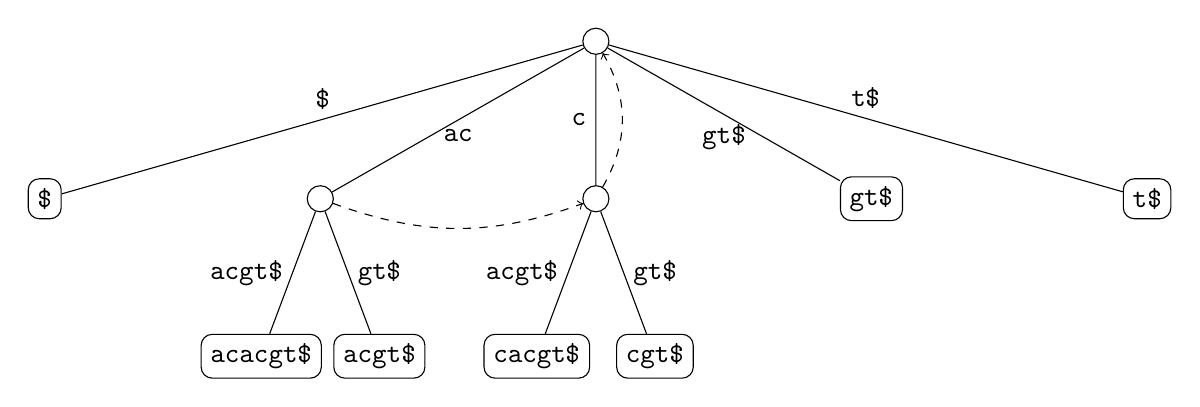
\begin{tikzpicture}
    [
        level 1/.style = {sibling distance = 3.5cm, level distance = 2cm},
        level 2/.style = {sibling distance = 1.5cm, level distance = 2cm}
    ]

        \node[draw, circle] (End2) {}
        child {
            node[draw, rounded corners] {\texttt{\$}}
            edge from parent node [above] {\texttt{\$}}
        }
        child {
            node[draw, circle] (Start1) {}
            child {
                node[draw, rounded corners] {\texttt{acacgt\$}}
                edge from parent node [left] {\texttt{acgt\$}}
            }
            child {
                node[draw, rounded corners] {\texttt{acgt\$}}
                edge from parent node [right] {\texttt{gt\$}}
            }
            edge from parent node [below] {\texttt{ac}}
        }
        child {
            node[draw, circle] (End1) {}
            child {
                node[draw, rounded corners] {\texttt{cacgt\$}}
                edge from parent node [left] {\texttt{acgt\$}}
            }
            child {
                node[draw, rounded corners] {\texttt{cgt\$}}
                edge from parent node [right] {\texttt{gt\$}}
            }
            edge from parent node [left] {\texttt{c}}
        }
        child {
            node[draw, rounded corners] {\texttt{gt\$}}
            edge from parent node [below] {\texttt{gt\$}}
        }
        child {
            node[draw, rounded corners] {\texttt{t\$}}
            edge from parent node [above] {\texttt{t\$}}
        }
        ;
        \draw[dashed, ->] (Start1) to[out=-20,in=200] (End1);
        \draw[dashed, ->] (End1) to[out=60,in=-60] (End2);
    \end{tikzpicture}
    \caption{Suffixboom voor de string \texttt{acacgt\$}. De stippellijnen stellen de suffix links voor.}\label{fig:suffix_tree_example}
\end{figure}

Natuurlijk is het niet efficiënt om de structuur op deze manier op te slaan.
Als de tekst lengte $n$ heeft, heeft de suffixboom ten hoogste $2n - 1$ toppen en $2n - 2$ bogen.
Het aantal toppen en bogen is dus $\Theta(n)$.
Jammer genoeg vraagt het opslaan van alle prefixen in de bladeren $\Theta(n^2)$ geheugen~\cite{AD3_ukkonen}.
We kunnen dit oplossen aan de hand van pointers naar het begin en einde van een substring in de originele string.
Hierdoor moeten we \textbf{geen kopie} meer opslaan\textbf{ van de originele string in elk blad}.
Sterker nog, we moeten dit zelfs niet in elk blad bijhouden.
We kunnen bij elke boog tussen de toppen labels bijhouden.
Het label van het blad kunnen we daarna reconstrueren door de labels van de bogen op weg naar dit blad achter elkaar te plaatsen.
Op deze manier wordt de nodige opslag per top een constante en krijgen we \textbf{lineair geheugengebruik} ($O(n)$).
Figuur~\ref{fig:suffix_tree_example_indices} toont hoe dit er in de praktijk uitziet.
Merk op dat indexering start vanaf nul en dat de eindindex exclusief is.
Een boog met waarde \texttt{1,3} stelt dus de substring \texttt{ca} voor uit het voorbeeld.
\begin{center}
    \texttt{tekst: a|c|a|c|g|t|\$\\index: 0|1|2|3|4|5|6}
\end{center}

\begin{figure}[H]
    \center
    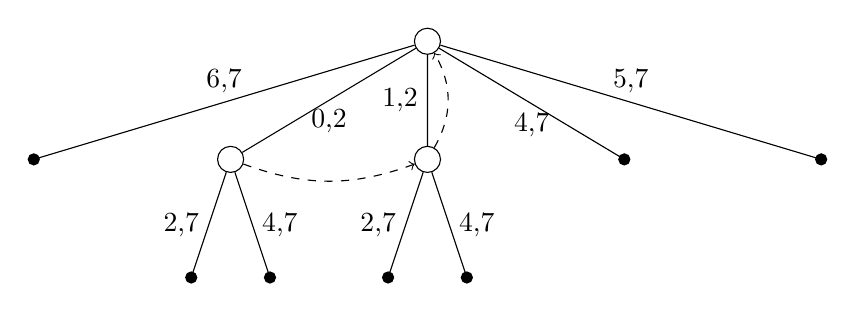
\begin{tikzpicture}
    [
        level 1/.style = {sibling distance = 2.5cm},
        level 2/.style = {sibling distance = 1cm}
    ]

        \node[draw, circle] (End2) {}
        child {
            [fill] circle (2pt)
            edge from parent node [above] {6,7}
        }
        child {
            node[draw, circle] (Start1) {}
            child {
                [fill] circle (2pt)
                edge from parent node [left] {2,7}
            }
            child {
                [fill] circle (2pt)
                edge from parent node [right] {4,7}
            }
            edge from parent node [below] {0,2}
        }
        child {
            node[draw, circle] (End1) {}
            child {
                [fill] circle (2pt)
                edge from parent node [left] {2,7}
            }
            child {
                [fill] circle (2pt)
                edge from parent node [right] {4,7}
            }
            edge from parent node [left] {1,2}
        }
        child {
            [fill] circle (2pt)
            edge from parent node [below] {4,7}
        }
        child {
            [fill] circle (2pt)
            edge from parent node [above] {5,7}
        }
        ;
        \draw[dashed, ->] (Start1) to[out=-20,in=200] (End1);
        \draw[dashed, ->] (End1) to[out=60,in=-60] (End2);

    \end{tikzpicture}
    \caption{Suffixboom voor de string \texttt{acacgt\$}, gebruikmakende van indices. De stippellijnen stellen de suffix links voor.}\label{fig:suffix_tree_example_indices}

\end{figure}

Deze suffixbomen laten toe om in $O(n)$ tijd substrings te zoeken binnen één string.
Hierbij is $n$ de lengte van de gezochte substring.
Indien we ook willen weten hoeveel voorkomens er exact zijn, en waar deze zich bevinden neemt dit $O(k)$ extra tijd.
Hierbij is $k$ het aantal voorkomens van de substring in de tekst.
Zoals eerder vermeld willen we echter peptiden zoeken in een \textbf{verzameling van proteïnen}.
Daarom wordt gebruikgemaakt van een \textbf{veralgemeende suffixboom}.
Hierbij wordt de verzameling van proteïnen die geïndexeerd moet worden behandeld alsof het één grote tekst is.
De manier waarop deze tekst gevormd wordt is echter erg belangrijk.
Alle proteïnen moeten aan elkaar gehangen worden met ertussen een teken dat niet in de proteïnen en peptiden zelf voorkomt.
Als eindteken moet er een ander uniek teken gebruikt worden.
Wanneer niet aan de eerste voorwaarde voldaan wordt, zullen we ongeldige matches vinden.
Het zou namelijk mogelijk zijn om een match te vinden die over twee of meer proteïnen gespreid is.
Wanneer niet aan de tweede voorwaarde voldaan wordt, dan breken we de eigenschap van suffixbomen waarbij elke suffix nooit een prefix van een andere suffix is.
Dit zou als gevolg hebben dat niet elke suffix een eigen blad in de boom krijgt.

\section{Het algoritme van Ukkonen}\label{sec:Ukkonen}
Het algoritme van Ukkonen~\cite{Ukkonen1995} is een complexe, maar efficiënte manier om suffixbomen op te bouwen in lineaire tijd met lineair geheugengebruik.
De beschrijving in de originele paper is vrij theoretisch, wat het algoritme minder toegankelijk maakt.
Het komt echter uitgebreid aan bod in een aantal andere publicaties en boeken~\cite{Gusfield1997, AD3_ukkonen, CCB_course, Ukkonen_CCB}.
Deze vormden een grote hulp bij het maken van een eigen implementatie.

\subsection{Kotlin}\label{subsec:kotlin}
Een eerste implementatie\footnote{\url{https://github.com/BramDevlaminck/SuffixTree}} van Ukkonen's algoritme heb ik met behulp van de programmeertaal Kotlin gemaakt.
Hierdoor kon er gefocust worden op het algoritme zonder belemmerd te worden door restricties opgelegd door de \textit{borrow checker}\footnote{\url{https://doc.rust-lang.org/1.8.0/book/references-and-borrowing.html}} van Rust.
Tijdens het implementeren was de referentiecode van prof.~Jan Fostier~\cite{Ukkonen_CCB} een groot hulpmiddel, omdat we hierdoor tijdens het debuggen het verloop van het programma konden opvolgen.
\\ \\
Het belangrijkste verschil tussen de Kotlin-implementatie en de referentie-implementatie is de manier waarop de kinderen voorgesteld worden.
Bij de eerste is dit aan de hand van een HashMap terwijl de laatste gebruikmaakt van een pointer array.
De reden voor de eerste aanpak is om alles zo simpel mogelijk te houden.
Hierdoor kon een karakter rechtstreeks als sleutel gebruikt worden, en was een omzetting naar een index niet nodig.
Om dit prototype te maken, heb ik gekozen voor Kotlin boven Python aangezien Kotlin performanter is en ook een aangename ontwikkelingservaring biedt.
Hierdoor is het mogelijk om de testdatasets op te bouwen binnen de 10 minuten.
\\ \\
Het grootste struikelblok tijdens het implementeren van het algoritme van Ukkonen waren enkele off-by-one fouten.
Aangezien je tijdens het algoritme werkt met substrings, maar deze opgeslagen worden aan de hand van hun begin- en eindindex, wordt het debuggen veel omslachtiger.
Tot slot had ik op het einde ook enkele bugs die niet voorkwamen in kleinere voorbeelden die met de hand uit te werken waren.
Dit maakte het lokaliseren en oplossen van de laatste problemen vrij tijdsintensief.

\subsection{Rust}\label{subsec:rust}
Door het \textit{ownership} systeem van Rust zijn er enkele belangrijke nuances in het implementeren van het algoritme van Ukkonen in Rust.
In de volgende secties bespreken we eerst enkele van deze nuances en hoe deze zich vertalen in onze eigen implementatie\footnote{\url{https://github.com/BramDevlaminck/FastPeptideMatching/tree/master/suffixtree}}.
Daarna bespreken we de performantie op vlak van snelheid en geheugengebruik.

\subsubsection{Boomstructuren}
Deze quote komt rechtstreeks uit een Medium artikel~\cite{rust_difficulty_quote} en toont direct aan waarom het maken van een suffixboom in Rust niet-triviaal is.
\begin{quote}
    \textit{Rust is known to be notorious difficult when it comes to certain data structures like linked lists, trees, etc.}
\end{quote}
De oorzaak hiervoor ligt bij het \textit{ownership} systeem van Rust.
Dit systeem zorgt ervoor dat elk stukje data slechts één eigenaar kan hebben.
In dit geval kan dus \textbf{slechts één top een andere top opslaan}, of er een \textit{mutable reference} naar hebben.
Concreet wil dit dus zeggen dat slechts één top een \textit{pointer} kan hebben naar een andere top, met de toelating om die top aan te passen.
Dit is net wat nodig is tijdens het opbouwen van de boom, want er worden nog kinderen toegevoegd en toppen gesplitst.
Dit is een probleem aangezien ouders pointers naar kinderen moeten hebben, de kinderen een verwijzing naar hun ouder, en er dan ook nog eens pointers zijn voor de suffix links.
\\ \\
Als oplossing hiervoor introduceert Rust het \texttt{Rc<T>} datatype.
Hierbij stapt Rust af van zijn standaard \textit{ownership} systeem en wordt gebruikgemaakt van \textbf{Reference Counting}~\cite{reference_counting}.
Pas wanneer alle referenties weg zijn, zal het geheugen automatisch vrijgegeven worden.
De beperking hierbij is echter dat deze referenties \textit{immutable} zijn.
Dit volstaat niet tijdens het opbouwen van de boom aangezien wij wijzigingen moeten kunnen maken aan de toppen waar naar verwezen wordt.
\\ \\
Om dit toch mogelijk te maken, introduceert Rust het \textbf{\textit{interior mutability}} patroon~\cite{interior_mutability}.
Hiervoor wordt gebruikgemaakt van het \texttt{Refcell} datatype.
Dit laat toe om data toch aan te passen, ook al is de referentie \textit{immutable}.
Aangezien dit de standaard Rust regels doorbreekt, is dit \texttt{unsafe}\footnote{Dit is code waarvan de compiler niet kan nagaan of die aan alle voorwaarden voldoet die nodig zijn om \textit{memory safety} te kunnen garanderen. Dit sleutelwoord bestaat zodat de programmeur meer vrijheid zou kunnen krijgen om bepaalde patronen toch te kunnen toepassen. De verantwoordelijkheid om correct het geheugen te gebruiken wordt hier bij de programmeur gelegd. Een andere reden om \texttt{unsafe} te gebruiken is om bepaalde interacties met hardware uit te voeren. Deze zijn inherent onveilig en zouden anders onmogelijk zijn.} en kan Rust \textit{at compile-time} geen \textit{memory safety} meer garanderen.
\texttt{Refcell} zal gelukkig de nodige code invoegen zodat runtime memory safety wel gegarandeerd is.
Mogelijke foutieve geheugenoperaties zullen dus tijdens het uitvoeren van het programma gedetecteerd worden, ten koste van performantie.
\\ \\
Maar zelfs dan blijft er nog altijd een probleem.
Geheugen dat beheerd wordt aan de hand van \textit{reference counting} zal enkel vrijgegeven kunnen worden indien de \textit{reference counter} op 0 staat.
Er zijn echter scenario's waar dit nooit zal gebeuren.
Namelijk bij \textbf{cyclische verwijzingen}; een patroon dat jammer genoeg erg vaak voorkomt.
In ons geval is dit een ouder die een pointer heeft naar een kind, dat zelf een pointer heeft naar die ouder.
Als oplossing hiervoor introduceert Rust dan weer het \texttt{Weak<T>} datatype.
\\ \\
De manier waarop Rust memory safety garandeert, introduceert duidelijk extra complexiteit en \textit{performance overhead} die ongewenst is en we willen vermijden.
Een optie zou kunnen zijn om expliciet het \texttt{unsafe} keyword te gebruiken, wat meer vrijheid geeft.
Het nadeel hiervan is natuurlijk dat we dan de garanties van memory safety kwijt zijn, wat net één van de hoofdredenen is om Rust te gebruiken.
Dit was dus geen optie.
Gelukkig is er een alternatieve manier waar ik op gestoten ben: een \textbf{\textit{arena-based} implementatie}~\cite{rust_arena_trees}.
Het idee hierbij is dat er één arena gemaakt wordt waarbij ownership erg simpel is.
In mijn implementatie is dit bijvoorbeeld een \texttt{Vector}.
Alle toppen worden hierbij in deze ene vector opgeslagen.
In plaats van pointers naar elkaar bij te houden, zullen de toppen getallen bijhouden.
Elk getal stelt de index van een top in de arena voor, waarnaar anders een pointer wordt bijgehouden.
\\ \\
Aangezien we alles in één vector opslaan, is het mogelijk om de nodige hoeveelheid geheugen onmiddellijk aan te vragen bij het opstarten van het programma.
Zoals in sectie~\ref{sec:wat-zijn-suffix-bomen?} beschreven staat zijn er ten hoogste $2n - 1$ toppen voor een tekst van lengte $n$.
Voor de Swiss-Prot databank die een inputstring van 206\thinspace523\thinspace693 karakters vormt, wil dit zeggen dat er in het slechtste geval 413\thinspace047\thinspace385 toppen zijn.
In de praktijk worden er echter slechts 328\thinspace922\thinspace516 toppen gevormd.
Indien we het geheugen op voorhand aanvragen zou het geheugengebruik dus nog met een factor $\frac{413\thinspace047\thinspace385}{328\thinspace922\thinspace516} \approx 1.26$ hoger liggen.
Daarom hebben we die aanpak niet gekozen.
\\ \\
Na het maken van deze ontwerpbeslissingen bleef slechts één moeilijkheid over.
Uitzoeken hoe de cursor (die bijhoudt waar we zijn in de boom tijdens het bouwen), de input string en de boom zich tot elkaar moeten verhouden in het systeem van eigenaarschap.
Uiteindelijk viel dit vrij makkelijk uit te zoeken, gebruikmakende van de foutmeldingen gegeven door \texttt{rustc}\footnote{De compiler voor de Rust programmeertaal}.
Het omzetten van de resterende Kotlin-code naar Rust was erg simpel en bijna een één-op-één vertaling.
Hier heb ik er echter voor gekozen om kinderen voor te stellen op dezelfde manier als in de C++-referentiecode.
Er wordt dus een array bijgehouden per top waarin plaats voorzien wordt voor alle mogelijke kinderen van die top.
Dit gebeurt ook indien een top geen, of slechts een klein aantal kinderen bevat.
Dit heeft als gevolg dat de \textbf{voorstelling van elke top even groot} is.

\subsubsection{Geheugenefficiëntie}
\textit{Null pointers} worden ook wel \textit{the billion-dollar mistake} genoemd vanwege het grote aantal bugs dat ze veroorzaken.
\begin{quote}
    \textit{And then I went and invented a null pointer.
    And if you use a null pointer you either have to check every reference or you risk disaster. \cite{null_mistake}}
\end{quote}
Daarom voorziet Rust een andere manier om de waarde \textit{null} voor te stellen.
Dit kan aan de hand van de \texttt{Option<T>} enum.

\begin{minted}{Rust}
enum Option<T> {
    None,
    Some(T),
}
\end{minted}

Deze enum heeft twee mogelijke waarden: \texttt{None} en \texttt{Some(T)}.
\texttt{None} is het equivalent van \textit{null}, terwijl \texttt{Some(T)} wil zeggen dat de waarde verschillend is van \textit{null}.
Meer specifiek heeft de waarde type \texttt{T}.
Aangezien het grootste deel van wat bijgehouden wordt per top pointers zijn, maakte ik veelvoudig gebruik van deze \texttt{Option} enum.
Alle pointers in een top kunnen namelijk \textit{null} zijn.
De \textit{parent pointer} moet nullable zijn aangezien de wortel geen ouder heeft.
Al zou dit wel elegant opgelost kunnen worden door de \textit{parent pointer} van de wortel naar zichzelf te laten wijzen.
De \textit{child pointers} moeten allemaal nullable zijn omdat bladeren geen kinderen hebben en in de interne toppen zijn niet alle kinderen altijd nodig.
Tot slot moeten de suffix links nullable zijn aangezien niet elke top een suffix link heeft naar een andere top.
\\ \\
Dit werkt perfect en kon mooi afgehandeld worden op de idiomatische manier die overeenkomt met goede Rust-code.
Na de eerste benchmarks bleek het \textbf{geheugengebruik} echter \textbf{problematisch}.
Bijna exact \textbf{2\times\ zo hoog als de equivalente C++ implementatie}.
Om zo'n drastisch verschil in geheugengebruik te kunnen verklaren, moest er wel iets fundamenteel verschillen aan de manier waarop toppen hun data bijhouden.
Al snel bleek dat het gebruik van \textbf{\texttt{Option<usize>}}\footnote{\texttt{usize}: \textit{The pointer-sized unsigned integer type \cite{usize}}. De grootte van dit datatype is het aantal bytes nodig om een referentie naar elk mogelijke locatie in het geheugen bij te kunnen houden. Voor 32- en 64-bit machines zijn dit resp.~4 en 8 bytes.} de boosdoener was.
Het gebruik van \texttt{Option<>} zorgt namelijk voor \textbf{8 bytes aan overhead}.
Aangezien een \texttt{usize} 8 bytes groot is op een 64-bit machine, verklaart dit inderdaad de verdubbeling van het geheugengebruik.
Dit valt makkelijk te controleren aan de hand van de \texttt{std::mem::size\_of} functie, deel van de Rust standaardbibliotheek.
\begin{minted}{Rust}
assert_eq!(mem::size_of::<Option<usize>>(), 16);
assert_eq!(mem::size_of::<usize>(), 8);
\end{minted}

Als oplossing heb ik uiteindelijk mijn \textbf{eigen \textit{null} waarde gedefinieerd} die gebruikmaakt van een \textit{trait}\footnote{Een trait in Rust definieert een functionaliteit die een bepaald type heeft, en kan delen met andere types.}.
Deze oplossing doet volledig het doel van de \texttt{Option<T>} enum teniet, maar is jammer genoeg nodig omdat het gewoonweg niet acceptabel is om het geheugengebruik hiervoor te verdubbelen.
Bovendien blijft \textbf{memory safety gegarandeerd}, aangezien het foutief indexeren van de null value (\texttt{usize::MAX} in dit geval) een index-out-of-bounds error genereert.
Dergelijke indexeringsfouten worden tijdens het uitvoeren gedetecteerd en geven dus geen verdere problemen (afgezien van een mogelijke crash van het programma).
\newpage
\begin{minted}{Rust}
/// Custom trait implemented by types that have a value that represents NULL
pub trait Nullable<T> {
    const NULL: T;

    fn is_null(&self) -> bool;
}

/// Type that represents the index of a node in the arena part of the tree
pub type NodeIndex = usize;

impl Nullable<NodeIndex> for NodeIndex {
    /// Use usize::MAX as NULL value since this will in practice never be reached.
    /// It is not possible to create 2^64-1 nodes (on a 64-bit machine).
    /// This would simply never fit in memory
    const NULL: NodeIndex = usize::MAX;

    fn is_null(&self) -> bool {
        *self == Self::NULL
    }
}
\end{minted}

\subsection{Performantie}\label{subsec:performantie}
Natuurlijk is het belangrijk dat de implementatie performant en correct is.
Aangezien we ook over een bestaande C++ implementatie van Ukkonen's algoritme beschikken, was dit een perfecte maatstaf om mee te vergelijken.
Uiteindelijk heb ik één aanpassing moeten maken in deze C++ code om een eerlijke vergelijking uit te voeren.
Oorspronkelijk werd er in elke top ruimte voorzien voor 256 mogelijke kinderen.
Dit was veel te hoog voor onze usecase.
Er zijn namelijk slechts 20 aminozuren en enkele \textit{wildcard characters}.
Dit verklaart onmiddellijk waarom het geheugengebruik initieel ongeveer tien keer hoger hoger was dan nodig.
Uiteindelijk ben ik gegaan voor een implementatie (zowel in Rust als C++) waar plaats is voor \textbf{28 kinderen}.
De 26 letters van het alfabet en de karakters \texttt{\#} en \texttt{\$}.
\texttt{\#} en \texttt{\$} die gebruikt worden als resp.~scheidingsteken en eindteken in veralgemeende suffixbomen.
Dit is ook wat al gebeurde in de bestaande C++ implementatie.
De exacte waarden van het scheidings- en eindteken zijn niet belangrijk, de enige eigenschappen die ze moeten hebben is dat ze niet voorkomen als teken in de proteïnen of peptiden, en verschillend zijn van elkaar.
\\ \\
Een andere aanpak zou kunnen zijn om HashMaps te gebruiken.
Het totale geheugengebruik zal hierdoor afnemen naar ongeveer 60\% van het huidige verbruik.
Dit gaat echter ten koste van performantie tijdens het zoeken, aangezien voor elke opvraging van een kind een hash berekend moet worden.
Hoe dan ook blijft het \textbf{geheugengebruik extreem hoog}, welke implementatie ook gekozen wordt.
\\ \\
Het vergelijken van de implementaties heb ik opgesplitst in twee stukken:
\begin{enumerate}
    \item Het opbouwen van de indexstructuur.
    Hierbij ligt de hoofdfocus op de indexgrootte aangezien deze de primaire beperkende factor is.
    \item Zoeken in de indexstructuur.
    Hierbij ligt de focus op de snelheid van het zoeken.
\end{enumerate}

\subsubsection{Opbouwen}
Om een representatief resultaat te krijgen, kijken we steeds naar het gemiddelde van 10 uitvoeringen.
De uitvoeringstijd en het geheugengebruik zijn gemeten aan de hand van het Unix \texttt{time} commando.
De resultaten hiervan zijn terug te vinden in Figuur~\ref{fig:tree_building}.
\begin{figure}[H]
    \centering
    \subfloat[Tijd nodig om de suffixboom op te bouwen.]{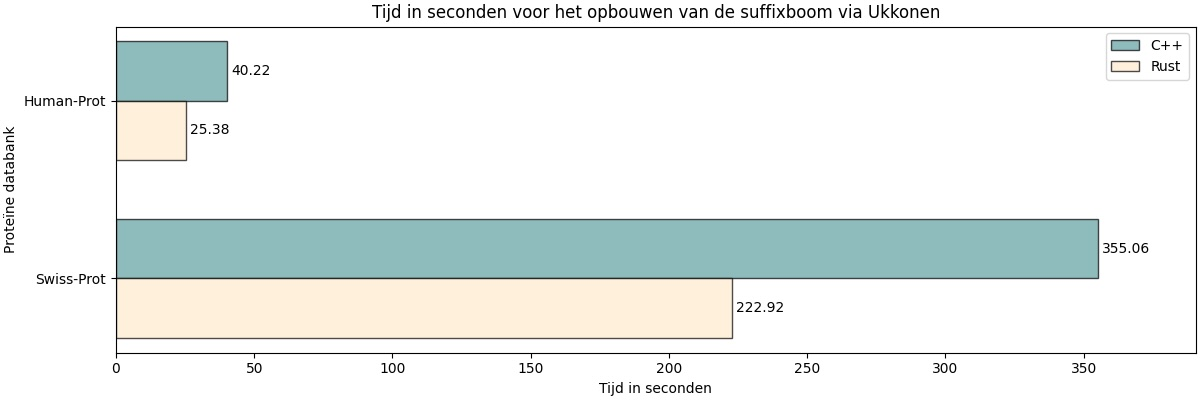
\includegraphics[width=\linewidth]{building_tree_time}}\\[4ex] % [4ex] om wat extra vertical spacing in te voegen

    \subfloat[Maximaal gebruikt geheugen tijdens het opbouwen van de suffixboom.]{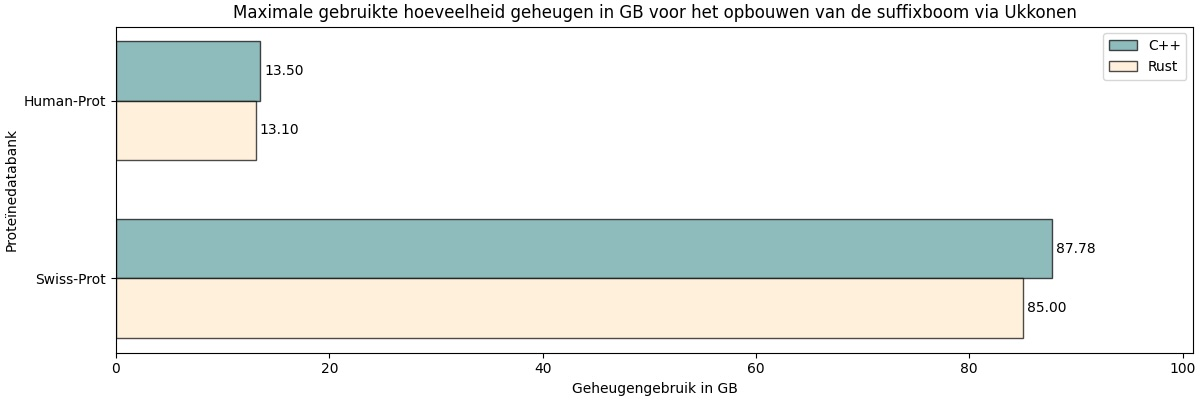
\includegraphics[width=\linewidth]{building_tree_memory}}
    \caption{Vergelijking tusen C++ en Rust implementaties voor het opbouwen van de suffixboom a.d.h.v.~het algoritme van Ukkonen. De tijd en het geheugengebruik zijn gemeten met het Unix \texttt{time} commando. Als invoerbestand gebruiken we hier de Swiss-Prot en Human-Prot proteïnedatabank.}\label{fig:tree_building}
\end{figure}

Uit deze grafieken vallen twee duidelijke conclusies te trekken.
\begin{enumerate}
    \item De implementatie in Rust is $\pm$ 33\% sneller.
    \item Het geheugengebruik is erg vergelijkbaar.
    Dit valt te verwachten aangezien beide implementaties 8 bytes nodig hebben per \textit{pointer} en evenveel plaats voorzien voor de kinderen.
    Het kleine verschil valt te verklaren vanwege één veld uit de C++ implementatie dat niet bijgehouden wordt in de Rust implementatie.
    Dit veld is de diepte van de top in de boom.
    Op de enkele plaatsen waar dit nodig is, kan gebruikgemaakt worden van andere variabelen om tot een equivalent resultaat te komen.
\end{enumerate}

\subsubsection{Zoeken}
Bij het zoeken zijn er twee belangrijke toepassingen om de snelheid te meten.
\begin{enumerate}
    \item Zoek totdat we weten of er een match bestaat voor de peptide.
    \item Zoek totdat er een match is, en doorzoek daarna de volledige subboom om alle informatie van de bladeren op te halen.

\end{enumerate}

\paragraph{Zoek een match}
Het meten van de zoektijd tot een match is een belangrijke indicatie van performantie, omdat bepaalde stukken informatie voorberekend kunnen worden voor elke top in de boom.
Hiervoor wordt informatie uit de bladeren tot aan de top van de boom gepropageerd.
In ons geval is dit bijvoorbeeld de LCA\footnote{Lowest Common Ancestor, Laagste Gemeenschappelijke Voorouder. Dit is de meest specifieke top in een boomstructuur (d.w.z.~de top zo diep mogelijk in de boom) die een ouder is van een elke top in de gegeven set van toppen.\label{footnote:lca}} van de taxon IDs.
Dit laat toe om het zoekproces te stoppen zodra er een match is.
De top waarin het zoeken stopt, zal de voorberekende LCA waarin we geïnteresseerd zijn bevatten.
Dit is de LCA van de taxa die horen bij de proteïnen waarvan de gezochte peptide een substring is.
\\ \\
Figuur~\ref{fig:performance_match_tree} toont de nodige tijd om alle peptiden van de gebruikte peptidebestanden éénmalig te zoeken totdat er een (mis)match was voor de peptide.
De grafiek bevat de gemiddelde resultaten van 5000 uitvoeringen, maar zelfs dan bleven de resultaten wat schommelen.
Doordat de te meten tijd zo klein is, kan de kleinste invloed van omgevingsfactoren al voor een zichtbaar verschil zorgen.
Dit kan bv.~een achtergrondproces zijn, maar ook invloed van een andere VM die op de fysieke machine bezig is.
Dit was ook merkbaar tijdens het testen, waar de verschillen tussen twee opeenvolgende uitvoeringen vaak groter waren dan het verschil tussen de C++ en Rust implementatie.
Toch kunnen we besluiten dat de \textbf{C++ implementatie een beetje performanter} is.
\\
\begin{figure}[ht]
    \centering
    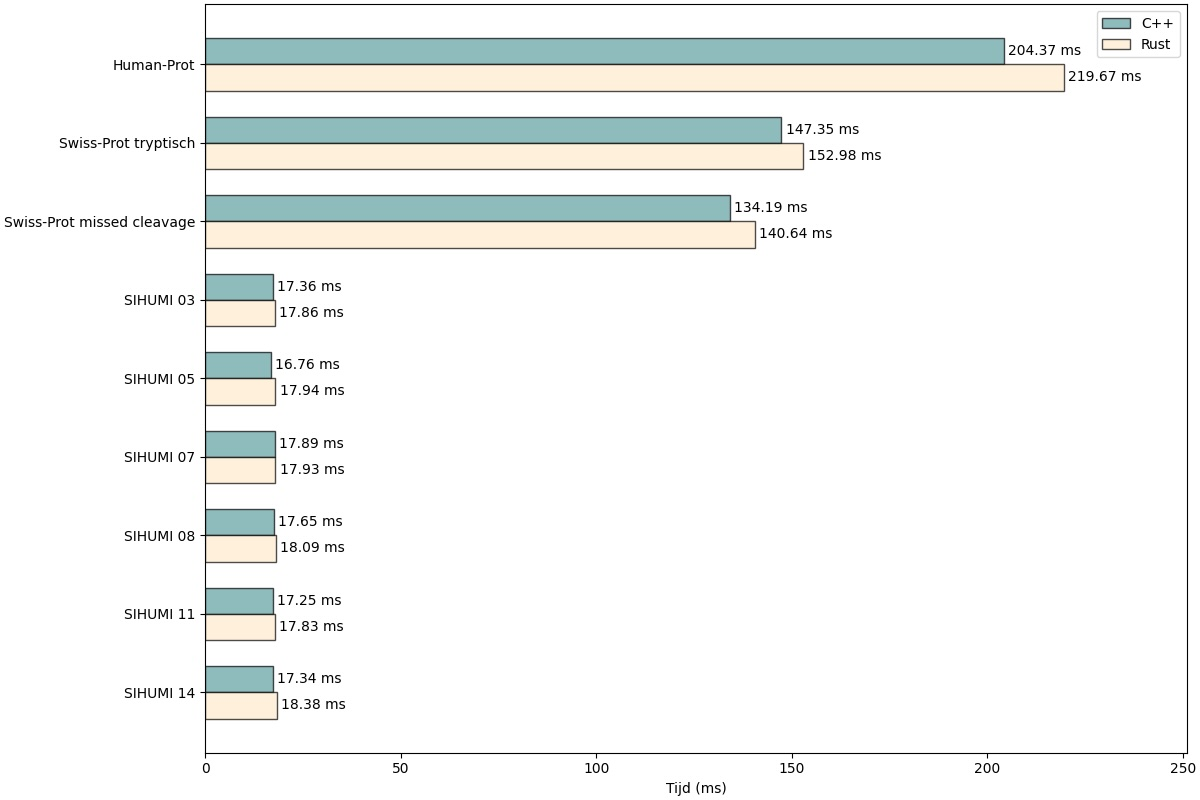
\includegraphics[width=\linewidth]{search_match_performance_tree}
    \caption{Uitvoeringstijd in milliseconden voor het zoeken tot een match voor alle peptidebestanden. Deze resultaten zijn het gemiddelde van 5000 uitvoeringen. Eén iteratie wordt gezien als eenmaal elke peptide die deel is van het peptidebestanden te zoeken in de suffixboom, en te stoppen wanneer er een (mis)match gevonden is. Het meten van de tijd is gebeurd in de code zelf.}
    \label{fig:performance_match_tree}
\end{figure}

Het verschil met de huidige implementatie van Unipept is aanzienlijk.
Daar duurt het op dit moment 2 minuten en 12 seconden om alle peptiden van het strikt tryptische Swiss-Prot peptidebestand te zoeken,
en maar liefst 30 minuten en 37 seconden voor het peptidebestand met \textit{missed cleavages}.
Dit is resp.~$\frac{132\thinspace000}{152.98} = 857$ en $\frac{1\thinspace837\thinspace000}{140.64} = 13\thinspace000$ keer trager.
Het gebruik van de suffixboom heeft echter ook nadelen ten opzichte van de huidige implementatie.
Deze laatste gebruikt slechts 6.7 GiB geheugen, en dit kan zelfs nog naar beneden.
Het geheugenverbruik tijdens het opbouwen van de huidige Unipept index wordt namelijk gedomineerd door een merge sort stap.
Het is mogelijk deze stap minder geheugen te geven, maar dan zal het sorteren wel langer duren.
De belangrijkste conclusie is echter dat de implementatie aan de hand van suffixbomen ongeveer 13 keer meer geheugen in neemt dan de huidige index.

\paragraph{Zoek match en haal informatie over kinderen op}
Indien we alle proteïnen willen vinden waar een peptide mee matcht, dan moeten we de volledige subboom doorzoeken, startende van de top waar de match eindigt.
De reden hiervoor is dat alle bladeren in deze subboom de gematchte proteïnen en de bijbehorende taxonomische informatie bevatten.
\\ \\
Figuur~\ref{fig:performance_all-occurrences_tree} bevat een overzicht van de nodige zoektijd voor beide implementaties op alle peptidebestanden.
We zien duidelijk dat er hier een \textbf{significant verschil is tussen de C++ en Rust implementatie}.
Vermoedelijk komt dit door de \textbf{andere \textit{memory layout}} die ontstaat doordat de Rust implementatie 1 grote vector gebruikt, terwijl de C++ implementatie losse toppen gebruikt die verspreid liggen in het geheugen.
Deze verbeterde lokaliteit zal het aantal cache-hits verhogen, wat op zijn beurt de performantie ten goede komt.

\begin{figure}[ht]
    \centering
    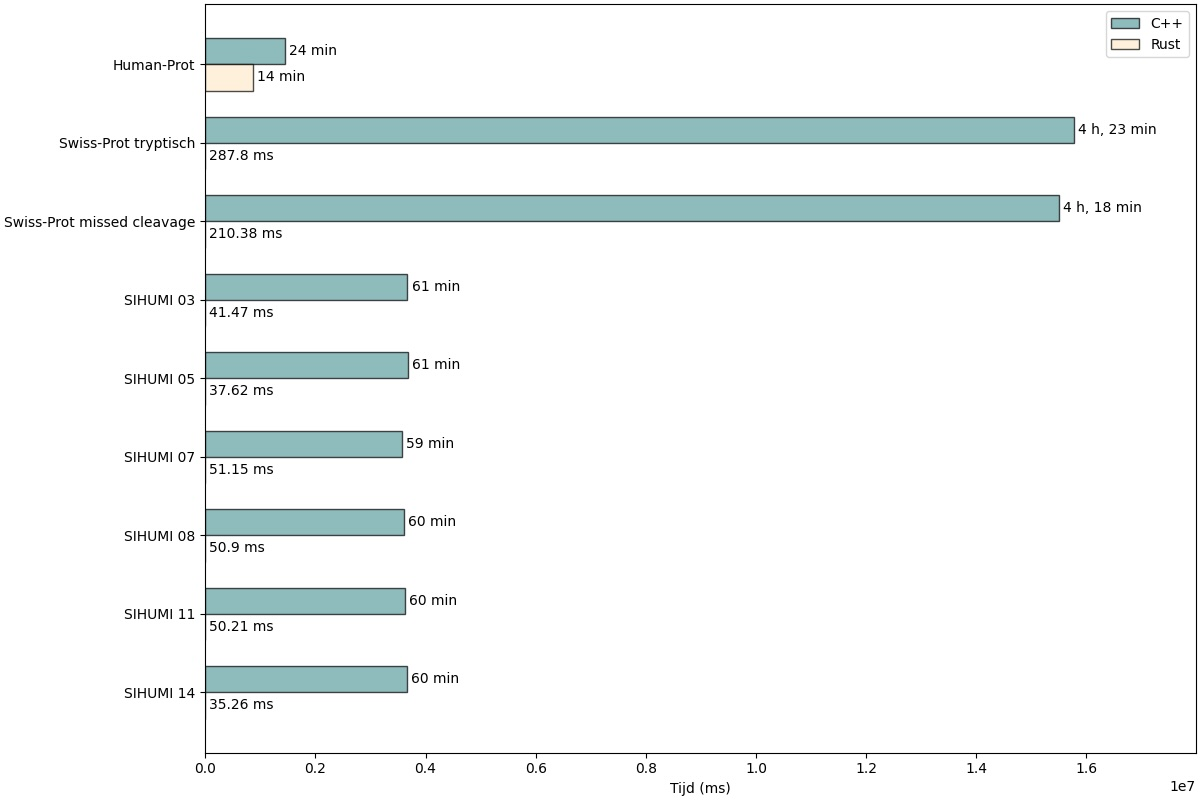
\includegraphics[width=\linewidth]{search_all-occurrences_performance_tree}
    \caption{Uitvoeringstijd inclusief het doorzoeken van de volledige subboom na match voor alle peptidebestanden. Deze resultaten zijn het gemiddelde van 10 uitvoeringen. Eén uitvoering wordt gezien als één keer elke peptide die deel is van het peptidebestand te zoeken in de suffixboom, en bij een match de volledige resterende subboom te doorzoeken. Dit toont de tijd die nodig is om informatie uit de bladeren op te halen voor alle proteïnen waar een peptide substring van is. Het meten van de tijd is gebeurd in de code zelf.}
    \label{fig:performance_all-occurrences_tree}
\end{figure}


\section{Taxon ID aggregatie}\label{sec:taxon-id-aggregatie}
Eén van de belangrijkste analyses die Unipept aanbiedt, is de \textbf{taxonomische analyse} waarbij uitgezocht wordt met welke organismen de peptiden uit een staal overeenkomen.
Aangezien peptiden kunnen matchen met proteïnen uit verschillende organismen, moet er een manier gekozen worden om deze \textbf{informatie te aggregeren}.
Een optie is om een schatting te maken en het organisme met de grootst mogelijke kans te nemen.
Unipept kiest echter voor een andere aanpak waarbij de informatie \textbf{conservatief} veralgemeend wordt.
Er is namelijk geen manier om met zekerheid te zeggen uit welke proteïne de peptide effectief komt.
Dit komt omdat gebruikers enkel een verzameling peptiden als input geven.
Geen extra info die toelaat om te snoeien zonder mogelijk correcte informatie te verliezen.
Anders gezegd: Unipept zal enkel info geven die geldt voor alle gematchte proteïnen.
Eén van deze stukjes informatie is het taxon ID\@.
Unipept zal niet de lijst van alle mogelijke taxon IDs teruggeven omdat dit twee nadelen heeft.
Ten eerste kan dit een erg grote lijst worden indien de peptide met erg veel proteïnen matcht.
Ten tweede zou dit ook vereisen om altijd de volledige subboom na een match te overlopen.
In plaats daarvan gaan we \textbf{via voorberekeningen de taxon IDs aggregeren gebruikmakende van de NCBI taxonomy\footnote{Dit is een boomstructuur die de evolutionaire relaties tussen organismen representeert. De laagste gemeenschappelijke voorouder van twee bladeren in deze boom representeert het evolutionair punt waarop deze twee organismen van elkaar afgesplitst zijn. Elke top in deze taxonomische boom heeft een uniek taxon ID, waarbij de wortel van de boom ID met waarde 1 heeft.} database}~\cite{NCBI_original_article, NCBI_update}.
Met andere woorden, we gaan op zoek naar de laagste gemeenschappelijke voorouder van alle taxon IDs die in de bladeren van de subboom zitten van een bepaalde top.
Hiervoor bestaan verschillende strategieën die al uitgewerkt zijn in UMGAP~\cite{UMGAP_paper, UMGAP_source}, en die hier herbruikbaar waren.
\\ \\
Initieel hebben we gekeken naar het LCA*\footnote{LCA = Lowest Common Ancester, Laagste Gemeenschappelijke Voorouder. De * wijst erop dat dit algoritme een variant is.} algoritme.
Dit is een heuristiek gebaseerd op de LCA\footref{footnote:lca}.
Bij LCA* zoeken we het meest specifieke taxon in de boom die ofwel een ouder of kind is van elke taxon in de boom.
Anders gezegd is dit de LCA van een verzameling taxa, nadat we alle taxa verwijderd hebben die ouder zijn van minstens één taxon in die verzameling~\cite{UMGAP_paper}.
Figuur~\ref{fig:lca*_example} legt dit uit aan de hand van een klein voorbeeld.
Het voordeel van LCA* ten opzichte van LCA is dat de resulterende data langer exact blijft.
De LCA van een verzameling van taxon IDs zal namelijk altijd als waarde 1 hebben, dus de root zijn, zodra één element in de verzameling als root geannoteerd is.
Dit gedrag willen we zo veel mogelijk vermijden.
\\
\begin{figure}[H]
    \centering
        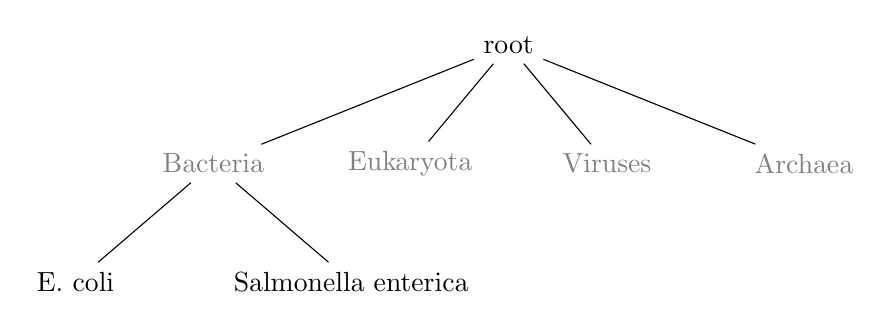
\begin{tikzpicture}
        [
            level 1/.style = {sibling distance = 2.5cm, level distance = 1.5cm},
            level 2/.style = {sibling distance = 3.5cm, level distance = 1.5cm}
        ]
            \node {root}
            child {node [gray] {Bacteria}
            child {node {E. coli}}
            child {node {Salmonella enterica}}}
            child {node [gray] {Eukaryota}}
            child {node [gray] {Viruses}}
            child {node [gray] {Archaea}}
            ;
        \end{tikzpicture}

    \caption{Sterk versimpelde voorstelling van de NCBI taxonomy. We berekenen de LCA en LCA* van de verzameling van zwarte toppen. De grijze toppen zijn \textit{placeholders}. De LCA van de verzameling \texttt{\{root, E. coli, Salmonella enterica\}} is vanzelfsprekend \texttt{root}, aangezien dit de wortel van de boomstructuur is. Bij het berekenen van de LCA* verwijderen we echter alle taxa die ouder zijn van minstens één taxon in de verzameling. \texttt{Root} is een ouder van zowel \texttt{E. coli} als \texttt{Salmonella enterica}, en wordt daarom niet gebruikt tijdens het berekenen van de LCA*. De LCA* wordt dus berekend door de LCA van de verzameling \texttt{\{E. coli, Salmonella enterica\}} te zoeken. Het resultaat hiervan is de top \texttt{Bacteria}. Dit illustreert hoe LCA* beter overweg kan met ``te algemene'' taxonomische annotaties.}
    \label{fig:lca*_example}
\end{figure}

Om het geaggregeerde taxon ID van elke interne top in de boomstructuur efficiënt voor te berekenen, was het idee om dit te doen op basis van de directe kinderen van die top.
Hiermee bedoelen we de eerstegraads kinderen.
Deze liggen één niveau lager in de boomstructuur, en hebben als ouder allemaal dezelfde top waarvan we het taxon ID willen berekenen.
De andere, tragere optie is om dit te doen op basis van de bladeren van de subboom van de top.
Door het te doen aan de hand van de directe kinderen van de top kunnen we in één bottom-up sweep van de boom alle taxon IDs berekenen.
Dit bleek echter niet mogelijk in combinatie met LCA* omdat gebruikmaken van de directe kinderen een ander resultaat geeft dan gebruikmaken van de bladeren van de subboom.
Figuur~\ref{fig:lca*_diff} toont een minimaal voorbeeld uitgewerkt voor beide strategieën.
De lichtgrijze toppen zijn ingevuld aan de hand van aggregatie, terwijl de zwarte toppen gegeven zijn.
Onderstaande uitleg behandelt de werkwijze bij beide opties.
\begin{itemize}
    \item Het toepassen van LCA* voor het berekenen van de top op basis van de bladeren van de boom (\{9606, 10566, 9606\}) heeft als resultaat 1 voor de wortel van de boom.
    9606 en 10566 zijn geen ouder of kind van elkaar, dus zal LCA* hetzelfde doen als LCA\@.
    De kleinste gemeenschappelijke ouder van deze twee taxa is 1.
    \item Het toepassen van LCA* op basis van de directe kinderen geeft als resultaat 9606.
    Dit valt simpel te verklaren aangezien de LCA* van de linker subboom 1 is.
    Als we daarna dan de LCA* van \{1, 9606\} nemen, wordt 1 verwijderd.
    Aangezien dit een ouder is van 9606.
    De LCA van 9606 is gewoon zichzelf.
\end{itemize}

\begin{figure}[h]
    \centering
    \subfloat[LCA* op basis van de bladeren.]{
        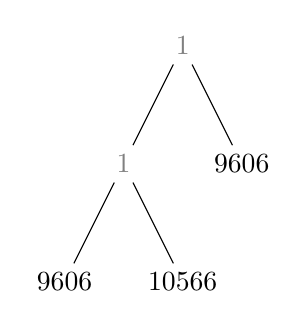
\begin{tikzpicture}
            \node [gray] {1}
            child {node [gray] {1}
            child {node {9606}}
            child {node {10566}}}
            child {node {9606}
            };
        \end{tikzpicture}
    }\hspace{0.25\textwidth}%
    \subfloat[LCA* op basis van de kinderen.]{
        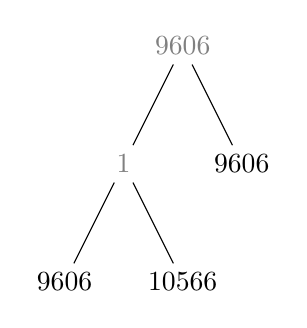
\begin{tikzpicture}
            \node [gray] {9606}
            child {node [gray] {1}
            child {node {9606}}
            child {node {10566}}}
            child {node {9606}
            };
        \end{tikzpicture}
    }
    \caption{Minimaal voorbeeld van de 2 aggregatiestrategieën gebruikmakende van LCA*. De grijze toppen zijn berekend aan de hand van een LCA*, terwijl de zwarte toppen gegeven zijn. In de NCBI databank stelt het organisme met NCBI taxon ID 10566 het \textit{Human papillomavirus} voor, organisme met ID 9606 de \textit{Homo sapiens} en ID 1 is een representatie van de wortel van de volledige NCBI taxonomy boomstructuur.}\label{fig:lca*_diff}
\end{figure}

Het berekenen van de \textbf{LCA* op de eerste manier is echter niet schaalbaar voor de volledige suffixboom}.
Om een idee van grootorde te geven: de suffixboom voor de Swiss-Prot dataset bevat in totaal 328\thinspace922\thinspace516 toppen, waarvan 206\thinspace523\thinspace693 bladeren.
\\ \\
Daarom hebben we \textbf{voorlopig toch voor de standaard LCA aggregatie manier} gekozen.
Deze laat wel toe de toppen op deze efficiëntere manier te aggregeren.
UMGAP biedt 2 implementaties aan om de LCA te berekenen voor een gegeven verzameling van taxa.
Gebruikmakende van RMQs\footnote{Range Minimum Queries} of een boomstructuur.
Mijn implementatie maakt gebruik van de RMQ implementatie aangezien deze significant sneller is (8 min 58 sec vs 20 min en 25 sec voor de Swiss-Prot databank) in mijn toepassing.
Tot slot heb ik voor Swiss-Prot ook eens vergeleken hoe groot de behaalde tijdswinst is als we de LCAs aggregeren aan de hand van de directe kinderen, vergeleken met aggregatie op basis van de bladeren.
Bij het aggregeren op basis van de bladeren met de RMQ implementatie was de uitvoeringstijd maar liefst 12 uur, 19 minuten en 16 seconden.
Dit is dus een extreem groot verschil.

\section{Conclusie}\label{sec:conclusie-suffix-bomen}
Het is duidelijk dat suffixbomen erg \textbf{performant} zijn voor het zoeken van willekeurige peptiden in een grote verzameling van proteïnen.
Zelfs als we alle bladeren onder een interne knoop voor een match willen afgaan, valt dit mee.
Bovendien is ook het opbouwen van de indexstructuur iets wat relatief snel gaat.
\\ \\
Door de eigen \textbf{implementatie in Rust}, kunnen we ook wat tijd besparen ten opzichte van een equivalente C++ implementatie.
Een deel van de \textbf{tijdswinst} zit in het\textbf{ opbouwen van de boom}, maar vooral tijdens het zoeken, wanneer \textbf{informatie uit de bladeren} gehaald moet worden.
Vermoedelijk ligt de andere geheugenstructuur hiervoor aan de basis.
\\ \\
Ondanks de veelbelovende resultaten op vlak van snelheid is er een keerzijde aan de medaille.
Het \textbf{geheugengebruik is zo groot dat we op zoek moeten naar een andere indexstructuur}.
Voor de Swiss-Prot databank gaat het geheugengebruik al boven 85 GB als we ook de taxon IDs voorberekenen, terwijl ons einddoel is om de indexstructuur op te bouwen voor de volledige UniProtKB databank.
Rekening houdende met het lineaire gedrag van het geheugengebruik wil dit zeggen dat alles nog $\pm$ 500 maal opgeschaald moet worden.
Dit zou echter vereisen dat we een server nodig hebben met ongeveer 45 TB aan RAM\@.
We hebben echter geen dergelijke machine ter beschikking.
Daarom moeten we op zoek naar andere indexstructuren die minder geheugen vereisen, eventueel met een impact op de zoeksnelheid.
In de praktijk hebben we namelijk wat marge om aan zoeksnelheid in te boeten, aangezien suffixbomen meerdere grootteordes sneller zijn dan de huidige Unipept index.
Een belangrijke voorwaarde hierbij is natuurlijk dat dit enkel acceptabel is als we hierdoor volledig UniProtKB kunnen indexeren.
